
\begin{figure}[Penalized elastic registration]{FIG:PENALTY}{Penalized elastic registration with different values of $\lambda$}
	\subfigure[SBFIG:PENALTY1]{Registration of $f_1$ to $f_2$ with a penalty term}{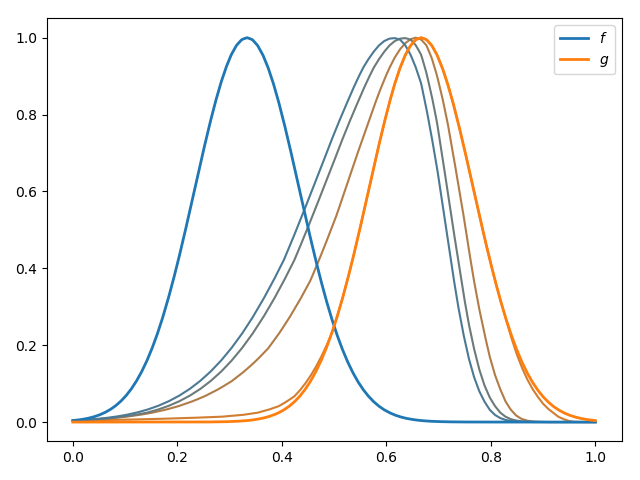
\includegraphics[width=7cm]{penalty-elastic}} \quad
	\subfigure[SBFIG:PENALTY2]{Warping used in the alignment}{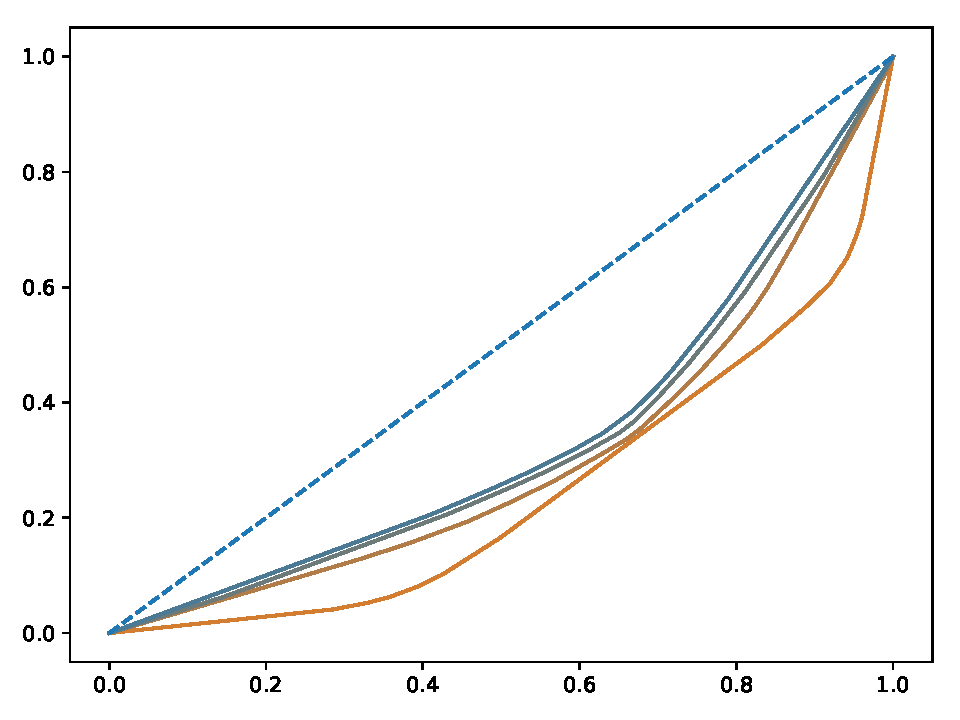
\includegraphics[width=7cm]{penalty-elastic-warping}}
\end{figure}

Sometimes it is necessary to control the amount of elasticity during the
registration process, for this purpose it is possible to add a penalty term
$\mathcal{R}(\lambda)$ to the elastic distance \ref{EQ:ELASTIC}.
Let $q_1, q_2 \in \mathbb{L}^2$ be two SRSFs and $\lambda > 0$, we will define
the penalized elastic distance as

\begin{equation}[]{Restricted amplitude distance}
d_{\lambda}\left(q_{1}, q_{2}\right) \equiv \inf _{\gamma \in \Gamma}\left(
\| q_{1}-\left(q_{2} \circ \gamma \sqrt{\dot{\gamma}}\right)\left\|^{2}+
\lambda\right\| \sqrt{\dot{\gamma}}-1 \|^{2} \right)^{(1 / 2)}.
\end{equation}

Once the registration process of our data has been completed,
we can proceed to another parts in the analysis of the data.
Regression and classification are two of the most important problems in
statistics, and therefore in \acs{FDA}.
Among the models to address these tasks are the nearest neighbors estimators,
which can be generalized directly to functional data. In the following section
is made a brief overview of these estimators.

%The alignment of two functions with different penalties is shown in the Figure \ref{FIG:PENALTY}.
